\documentclass[10pt,twocolumn,letterpaper]{article}

\usepackage{cvpr}
\usepackage{times}
\usepackage{epsfig}
\usepackage{graphicx}
\usepackage{amsmath}
\usepackage{amssymb}
\usepackage{array}
\usepackage{xfrac}
\usepackage{amssymb}
%\usepackage{todonotes}
\usepackage{centernot}
\usepackage{textcomp}
\usepackage{blindtext}
\usepackage{centernot}
\usepackage{wasysym}
\usepackage{siunitx}
\usepackage[letterpaper]{geometry}
\usepackage{color}
%\usepackage[table]{xcolor}
\usepackage{amsfonts}
\usepackage{mathtools}
\usepackage{multirow}
\usepackage[small,it]{caption}
%\usepackage{titling}
%\usepackage{filecontents}
%\usepackage{titlesec}
\usepackage[section]{placeins}
%\usepackage[hidelinks]{hyperref}
%\usepackage{fancyhdr}
\usepackage{cancel}
%\usepackage{abstract}
\usepackage{minted}
\usepackage{widetext}
\usepackage[utf8]{inputenc}

\sisetup{output-exponent-marker=\textsc{e}}

\DeclareMathOperator*{\argmax}{arg\,max}
\DeclareMathOperator*{\argmin}{arg\,min}

\newcommand{\squishlist}{
 \begin{list}{$\bullet$}
  { \setlength{\itemsep}{0pt}
     \setlength{\parsep}{3pt}
     \setlength{\topsep}{3pt}
     \setlength{\partopsep}{0pt}
     \setlength{\leftmargin}{1.5em}
     \setlength{\labelwidth}{1em}
     \setlength{\labelsep}{0.5em} } }


\newcommand{\squishlisttwo}{
 \begin{list}{$\bullet$}
  { \setlength{\itemsep}{0pt}
    \setlength{\parsep}{0pt}
    \setlength{\topsep}{0pt}
    \setlength{\partopsep}{0pt}
    \setlength{\leftmargin}{2em}
    \setlength{\labelwidth}{1.5em}
    \setlength{\labelsep}{0.5em} } }

\newcommand{\squishend}{
  \end{list}  }
\footskip = 50pt
\setlength{\skip\footins}{10pt}

\newcommand*{\vertbar}{\rule[-1ex]{0.5pt}{3.0ex}}
\newcommand*{\horzbar}{\rule[.5ex]{2.5ex}{0.5pt}}

% Include other packages here, before hyperref.

% If you comment hyperref and then uncomment it, you should delete
% egpaper.aux before re-running latex.  (Or just hit 'q' on the first latex
% run, let it finish, and you should be clear).
\usepackage[breaklinks=true,bookmarks=false]{hyperref}

\cvprfinalcopy % *** Uncomment this line for the final submission

\def\cvprPaperID{****} % *** Enter the CVPR Paper ID here
\def\httilde{\mbox{\tt\raisebox{-.5ex}{\symbol{126}}}}

% Pages are numbered in submission mode, and unnumbered in camera-ready
%\ifcvprfinal\pagestyle{empty}\fi
\setcounter{page}{1}
\begin{document}

%%%%%%%%% TITLE
\title{Unsupervised Image Segmentation based on Clustering and Watersheds}

\author{Edgar A. Margffoy-Tuay\\
Universidad de los Andes\\
201412566\\
{\tt\small ea.margffoy10@uniandes.edu.co}
% For a paper whose authors are all at the same institution,
% omit the following lines up until the closing ``}''.
% Additional authors and addresses can be added with ``\and'',
% just like the second author.
% To save space, use either the email address or home page, not both
%\and
%Second Author\\
%Institution2\\
%First line of institution2 address\\
%{\tt\small secondauthor@i2.org}
}

\maketitle
%\thispagestyle{empty}

%%%%%%%%% ABSTRACT
\begin{abstract}
Unsupervised clustering methods allow not just only to cluster general information, they also can be used to produce a region segmentation of an input image, this approach allowed researchers to propose different procedures and pipelines to segment an image, from grouping pixels into superpixels, to evaluate its results on tasks of segmentation against evaluation methodologies, databases and benchmarks, such as the Berkeley Segmentation Dataset and Benchmark (BSDS500). The present report pretends to evaluate these methods against the latter tasks over a proposed cuantitative evaluation framework.
\end{abstract}

%Segmentation represents one of the core Computer Vision tasks in scientfic and academic research since the 1970s, this problem is defined as the grouping of pixels on a image according to several semantic categories of interest. Until recently, this problem was approached by using pixel-level mathematical formulations based on classical image processing and DSP, without any association with other Computer Vision problems nor any AI-related task, such as NLP. However, after the rise of

%%%%%%%%% BODY TEXT
\section{Introduction}
%\subsection*{Context}
Image segmentation and contour detection are closely related problems that rely on the same premise: Given an image, find a partition (Grouping) of this pixels according to the boundaries that compose it. From this premise, it is possible to treat a segmentation problem as a contour detection and viceversa, this approach allows to propose and define several procedures to solve and evaluate this problem. 
\\
\\
Before the introduction of supervised learning techniques to solve this problem, all the approaches and proposed solutions were restricted only to the pixel information present on the image (Unsupervised segmentation) which served as input to different algorithms that provided a higher order representation of the image (Superpixels) or even partial segmentation images. Of these afromentioned algorithms, it is worth to mention clustering-based methods, such as those based on classic generic clustering methods, such as K-Means, Gaussian Mixture Models, Hierarchical clustering (To be explained during the following section) and Mean Shift \cite{1000236}. Other important methods represent the image as a directed graph with weights in which a minimal cut between regions delimited by a contour is desired, an example of an algorithm present on this category corresponds to the Normalized Cuts framework proposed by Shi and Malik \cite{868688}. Finally, other method families try to represent the segmentation problem from a morphological perspective, in which the image is seen as an intensity surface that describes valleys and intensity peaks, in which, boundaries can be seen as inflection peaks, this is the base of the Watershed transform method \cite{Beucher1994}.
\\
\\
Although all the unsupervised methods yield reasonable results that group the pixels of an image into disjoint regions, these methods underperform the performance presented by the modern state-of-the-art supervised segmentation algorithms, which render the previously approach only of interest if a superpixel representation of an image is desired, also, some of the unsupervised models are suitable to semi-automatic applications, such as interactive segmentations.

\section{Materials and Methods}

%\begin{figure*}[t]
%	\centering
%	%	\begin{center}
%	%\fbox{\rule{0pt}{2in} \rule{0.9\linewidth}{0pt}}
%	\epsfig{file=./Assets/Model_red.pdf,width=0.8\linewidth,clip=}
%	%\includegraphics[width=0.8\linewidth]{egfigure.eps}
%	%	\end{center}
%	\caption{Visual description of the planned baseline to approach the image segmentation recovery problem given a video input. Images taken by the author}
%	\label{Fig:F1}
%	%\label{fig:long}
%	%\label{fig:onecol}
%\end{figure*}

\subsection*{About the Implementation}
A total of four unsupervised segmentation routines were implemented and subject to direct comparison by using the labels and ground truth masks defined by the evaluation methodology proposed for this purpose, by comparing the contours obtained by thresholding the boundaries present between regions after clustering an image with the reference contours present on the dataset. Three out of four methods are based on classical general-purpose clustering methods, namely, K-means, Gaussian Mixture Models and Hierarchical segmentation. Finally, the last method is based on hierarchical watersheds with extended h-minima imposition. 
\\
\\
With respect to the image input representation to each of the segmentation methods, it is possible to notice that due the difference between the implementation and purpose of the clustering methods and the morphological segmentation based on watersheds, the input representation may vary, to accomplish this task, the image was evaluated over several colorspaces (RGB, HSV and La$^{*}$b$^{*}$), however, to cluster this representation, it is necessary to unroll each pixel coordinate triplet \eqref{eq:rgbim} as a column vector, as described on \eqref{eq:repr}, in this case, the spatial coordinates maybe added to enforce spatial segmentation coherence and reduce the number of disjoint regions labeled to the same cluster without being in the same spatial area. Analogically, to process the image by employing the watershed transform, the grayscale gradient was calculated by using the Sobel derivatives, the flooding procedure was done over the image representation on any colorspace, without any spatial information. Finally, the contour detection and thresholding of the segmentation was done using the Canny edge detector.


\begin{widetext}
	\begin{alignat}{2}
	\begin{bmatrix}
	(R_{1,1}, G_{1,1}, B_{1,1}) & (R_{1,2}, G_{1,2}, B_{1,2}) & \cdots & (R_{1,n}, G_{1,n}, B_{1,n}) \\
	(R_{2,1}, G_{2,1}, B_{2,1}) & (R_{2,2}, G_{2,2}, B_{2,2}) & \cdots & (R_{2,n}, G_{2,n}, B_{2,n}) \\
	\vdots & \cdots & \ddots & \vdots \\
	(R_{m,1}, G_{m,1}, B_{m,1}) & (R_{m,2}, G_{m,2}, B_{m,2}) & \cdots & (R_{m,n}, G_{m,n}, B_{m,n})
	\end{bmatrix} \label{eq:rgbim}
	\end{alignat} 
	
	\begin{alignat}{2}
	\begin{bmatrix}
	R_{1,1} & R_{1,2} & \vertbar & R_{m,n} \\
	G_{1,1} & G_{1,2} & \vertbar & G_{m,n} \\
	B_{1,1} & B_{1,2} & \cdots & B_{m,n} \\
	1 & 1 & \vertbar & m \\
	1 & 2 & \vertbar & n
	\end{bmatrix} \label{eq:repr}
	\end{alignat} 
	
\end{widetext}   

The implementation of the watershed procedure is based on the OpenCV\footnote{\url{http://opencv.org}} Python bindings, with the regional minima extraction routines adapted from the Gala library\footnote{\url{https://github.com/janelia-flyem/gala}}, the clustering methods are based on the Sckit-learn\footnote{\url{http://scikit-learn.org/stable/}} implementations. Also, the centroid and means initialization for K-Means and GMM was based on the KMC$^{2}$\footnote{\url{https://github.com/obachem/kmc2}} algorithm \cite{Bachem:2016:AKS:3016100.3016103}, all the routines were implemented on Cython, to improve execution times and the efficiency of the evaluation procedure.



\subsection*{About the models}
\subsubsection*{K-Means}
In the present experiment, K-Means was employed to segment an image by conforming clusters from pixel information, the clusters means were calculated by using the $\ell_2$ distance metric (Euclidean), which gives rise to spherical and convex color clusters, which can be spatially sparse or localized, depending on the inclusion of spatial information. To segment an input image, for each color triplet, the label of the closest mean is assigned, finally, the segmented image is reshaped into the image original dimensions.

\subsubsection*{Gaussian Mixture Model (GMM)}
The GMM procedure pretends to explain the input image\footnote{It is assumed that its values are normally distributed} as the set of points spanned by a set of $K$ gaussian distributions. To fit the set of distributions, it is essential to find the maximum likelihood parameters of each gaussian, namely, its mean $\mu_k$ and its covariance matrix $\Sigma_{k}$. To maximize those parameters, the Expectation Maximization (EM) algorithm is employed, this routine employs the Mahalanobis distance to model the data, which implies that the distribution may present skewness and doesn't have to be spheric or symmetrical around each axis. The maximization of the a priori probability of the model given the data allows to assign a membership probability to each of the $K$ distributions to each value. In practice, the label of the distribution which have the greater probability is chosen. 

\subsubsection*{Hierarchical Clustering}
The hierarchical clustering allows to define segmentation regions by merging smaller pixel regions, which in turn are formed by joining other smaller pixel regions, until each pixel of the image corresponds to its own region. To accomplish this process of merging, it is necessary to define a similarity measure between groups, if the similarity is minimal between clusters, then both are merged and a new cluster is formed. Due to its hierarchical character, this model allows to group several segmentations, which in turn allows to evaluate and pick the best level. However, computing the similarity between clusters is a expensive operation which requires significant amounts of memory, this means that this procedure can't scale if the input dimension increases. During the present experiment, the Ward linkage was used to relate the clusters, this measure expresses that not just only the centroids of both clusters must be near to each other, but each value present in both sets must be near, this measure allows to join spatially close values if the spatial coordinates are included.
\\
\\
To obtain $K$ segmentation regions, the merging algorithm must be repeated until only $K$ groups are left. Due to the excessive memory consumption, each image had to be down scaled by a factor of 0.5, however, this implied a memory consumption of 12Gb, less than the 60Gb required to evaluate the original image. 

\subsubsection*{Watershed Transform}
The watershed transform is based on the concept of watershed lines, these lines correspond to the local basin in which all drops of water are gathered when they fall down from a peak. In this context, the peaks of the images correspond to contours, and the space between borders may correspond to a river basin, the idea of the algorithm is to flood the image from the river basins (Regional minima), up to the peaks, at the end of the procedure, only the peaks remain, which implies that a boundary segmentation of the image is achieved. However, due to the existance of multiple regional minima on the gradient, this method is prone to produce an oversegmentation of the image, to overcome this limitation, it is possible to define a set of precomputed markers and impose them over the image, by executing this procedure, the flooding is not done over the set of markers, reducing the oversegmentation on the image. Due to the inexistance of precomputed markers over each image, the markers are selected as the regional minima of height $h$ (h-minima), the value of $h$ is increased, starting on 0, until the total number of regions is equal to $K$.  

\section{Results}
To evaluate unsupervised methods applied to image segmentation, it was necessary to formulate a common evaluation ground, in which every method can be compared directly with other methods, to address this issue, a subset of eight images were sampled from the Berkeley BSDS Segmentation database, each image have four levels of segmentations, ranked according to the number of regions labeled, also each level contains its contour map ($y$). The evaluation procedure consists on taking the original image and for each of segmentation levels ($K$ regions), apply any colorspace, include or not include spatial information and then applying a segmentation method to obtain a segmentation that presents $K$ regions, then it is threshold and binarized to obtain a contour map ($\hat{y}$), which is compared to the ground truth employing the mean absolute difference \eqref{eq:acc}, this ensures that all possible combinations are evaluated, and a score calculated per each combination.

\begin{alignat}{2}
Acc &= 1 - \frac{||y - \hat{y}||}{||y + \hat{y}||} \label{eq:acc}
\end{alignat}

This evaluation method presents several shortcomings related to the comparison estimate between the ground truth contour map and the boundaries obtained via unsupervised segmentation, it may possible that the boundaries differ by a margin of one to four pixels, depending on the process of thresholding employed. This means that a segmentation result that is identical to the ground truth but presents a margin may have a large absolute difference, and by consequence, a low score. Another shortcoming of the evaluation criteria is related to the bounds of the result boundaries and the real borders, both must be on the same scale, to preserve the limit bounds of the mean absolute difference term and allow the accuracy to be calculated as a percentage.  
\\
\\
 With respect to K-Means (Figure~\ref{Fig:kmeans1}), it is possible to conclude that without spatial information, this is prone to group distant regions that present a similar color value on any space, this result may be relevant for other applications such as image compression but in the context of image segmentation this may degrade the performance of the method, which means that relying only on color information alone is not enough to ger a reasonable segmentation result. To account for this limitations, it is possible to include the spati nal coordinates to each input vector, however, this causes the appeareance of spherical localized regions, which implies that the final result of the segmentation is close to a Voronoi pattern, as it is shown on Figure~\ref{Fig:kmeans2}. Similar results were obtained when applying this method on other colorspaces with spatial information, convex clusters tend to form around the mean points, however, when color information is used alone, small details related to the boundaries and other interior regions go largely unnoticed. However, the importance of using different colorspaces radicates on the element composition of the image, if the image depends on color details, then it is possible to represent it through the LAB channels, whereas if the image depends on shades of the same color, then the HSV representation is more suitable. Due to the introduction of possible random regions and noise by effects of the convex region boundaries, the overall accuracy of the K-Means method was about 10\% (Subject to spatial information)
 \\
 \\
 During the evaluation process, the colormap did not impact on the accuracy results more than the introduction of spatial features to the models, for instance, the GMM model sensitivity to form skewed   and short distributions caused the interweaving of different segmentation regions on the image (Figure~\ref{Fig:gmm1}), result that introduced noise at the moment to threshold the segmentation and caused a low performance of the method (4.15\% Overall). However, with the introduction of spatial features, as can be seen on Figure~\ref{Fig:gmm2}, the interweaving noise was reduced, however, the performance score only increased to 5.2\%, which implies that noise persists.
 \\
 \\
 With respect to other factors that may affect the overall performance of each method, it was possible to conclude that downsampling an image to a lower dimension increases the loss of information, which degrades the quality of the segmentation, and by direct consequence, the boundary detection is noisy when the result is upsampled to the original size. For instance, this was a limitation found while evaluating the Hierarchic segmentation method, due to the image resize, the quality of the segmentations was poor and the process took a significant time (\~ 5min per color representation), which doesn't improve the process, although more resources are used. The hierarchic segmentation proved to be inefficient due to the expensive cost of the Ward's linkage calculation done over all the values of the image, which cost $\mathcal{O}((mn)^2)$ per level merged. Also the degradation of the image signal by downsampling impacts the final result, due to the noise introduction to the image by effects of interpolation. This method obtained an Overall score of 4\%
 \\
 \\
 Finally, the limitations associated to Watershed transformation of an image are related to the number of regions detected by using the h-minima approach, which caused to important regions to disappear when the total number of regions desired is too low, that implies that the process of finding h-regional minima favours to select those minima found on contours well defined, which are found in small regions, however, if the total number of regions increases, the watershed procedure produces well defined contours and regions that are proximate to the ground truth, also this method is less expensive to calculate than the clustering family of segmentation procedures, however, the dependence on the choice of markers represent one of the major shortcomings of this method. As it can be shown on Figure~\ref{Fig:water1}, the total number of regions allows to propose well defined regions and contours, however, decreasing the total number of desired regions removes the principal regions to discriminate, thus degrading the performance of the method (Figure~\ref{Fig:water2}), which in turn implies a total performance of 2\% Overall.  
 \\
 \\
After applying this methodology to the image set, it is possible to appreciate that the method that presents the best accuracy corresponds to K-Means, by the reasons previously exposed.

\section{Conclusions}
To segment an image by only using Unsupervised Methods represents a challenge due to the low control over the convergence and results of the procedure, which allows other factors such as the richness and completeness of the input data representation (Colorspace and spatial information) to influence the final result more than the model parameters. Overall, the family of unsupervised methods are versatile to form expressive groups and superpixels from ground data, however at the moment to being compared with human segmentations, there is a large gap, due to the heuristic character of the processes. However, it is possible to evaluate the fitness of these models to solve the segmentation problem under an well-defined evaluation methodology, which allows to propose cuantitative conclusions from the data. 



{\small
\bibliographystyle{ieee}
\bibliography{egbib}
}


\newpage
\section{Some Results}
\begin{figure}[H]
	\centering
	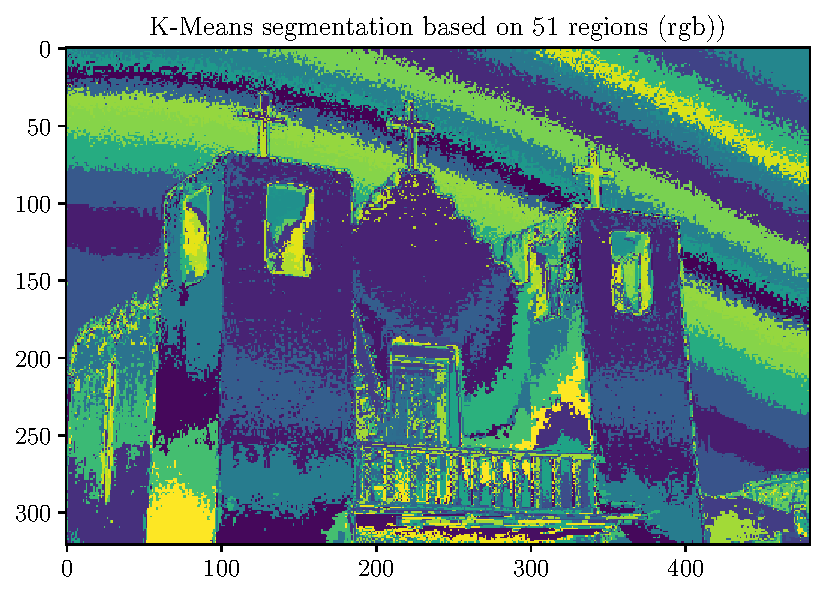
\epsfig{file=./Assets/24063_k-means_rgb_51.pdf,width=1.0\linewidth,clip=}
	\caption{Example of K-Means segmentation result subject to 51 regions (No spatial)}
	\label{Fig:kmeans1}
\end{figure}


\begin{figure}[H]
	\centering
	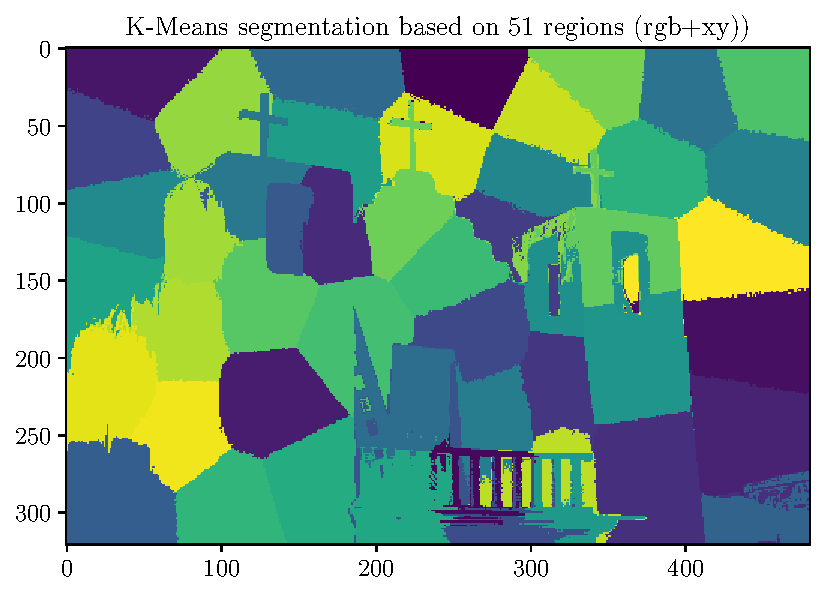
\epsfig{file=./Assets/24063_k-means_rgb+xy_51.pdf,width=1.0\linewidth,clip=}
	\caption{Example of K-Means segmentation result subject to 51 regions (Spatial), this figure presents a large number of convex and spherical regions}
	\label{Fig:kmeans2}
\end{figure}

\begin{figure}[H]
	\centering
	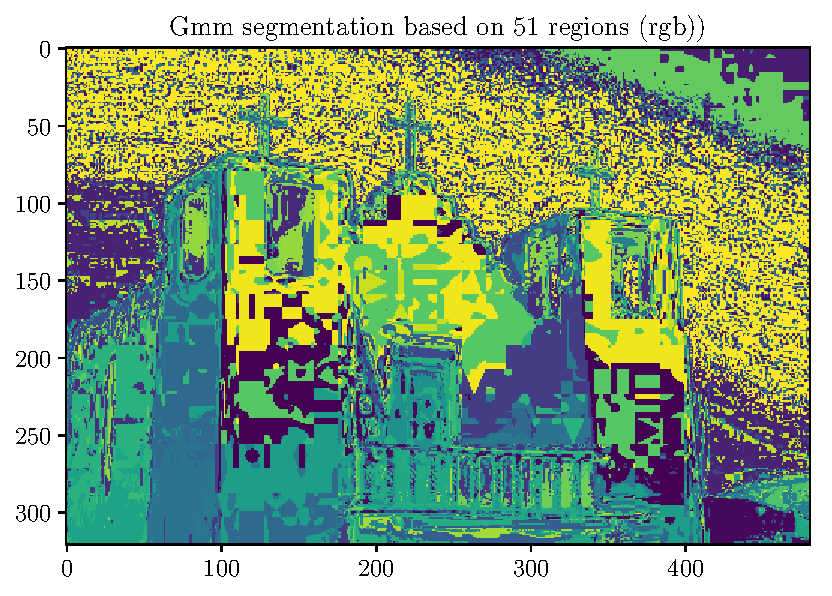
\epsfig{file=./Assets/24063_gmm_rgb_51.pdf,width=1.0\linewidth,clip=}
	\caption{Example of GMM segmentation result subject to 51 regions (No spatial)}
	\label{Fig:gmm1}
\end{figure}

\begin{figure}[H]
	\centering
	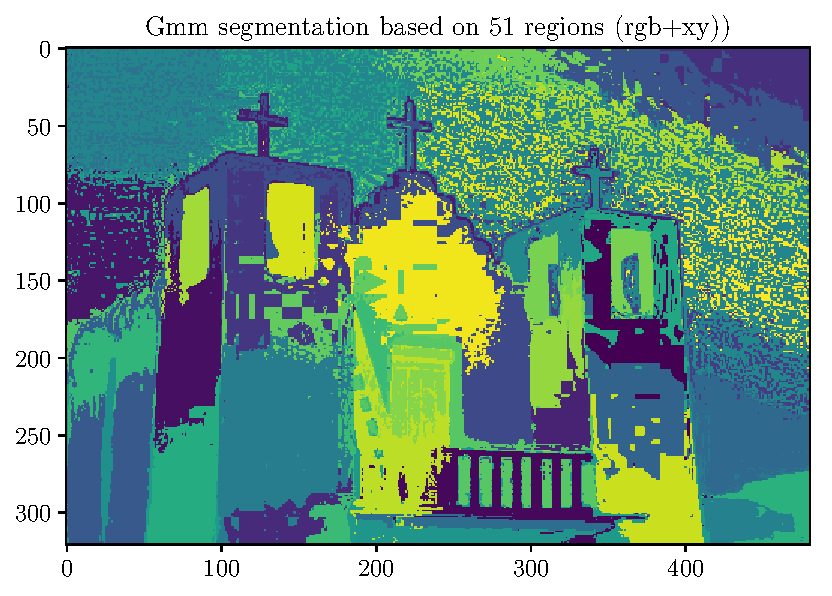
\epsfig{file=./Assets/24063_gmm_rgb+xy_51.pdf,width=1.0\linewidth,clip=}
	\caption{Example of GMM segmentation result subject to 51 regions (Spatial information added), the noise was reduced}
	\label{Fig:gmm2}
\end{figure}

\begin{figure}[H]
	\centering
	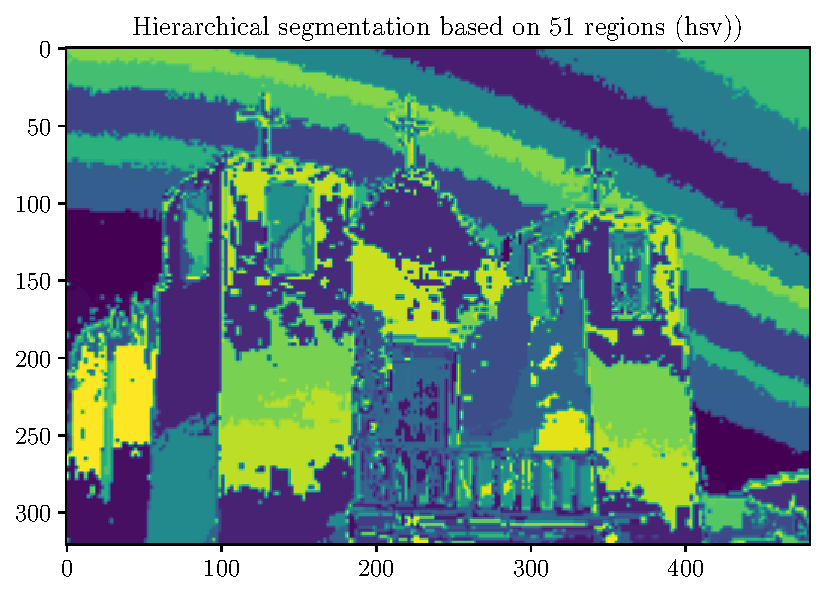
\epsfig{file=./Assets/24063_hierarchical_hsv_51.pdf,width=1.0\linewidth,clip=}
	\caption{Example of Hierarchic segmentation result subject to 51 regions (No spatial information added), notice the smooth noise throughout all the regions by interpolation effects}
	\label{Fig:hier1}
\end{figure}

\begin{figure}[H]
	\centering
	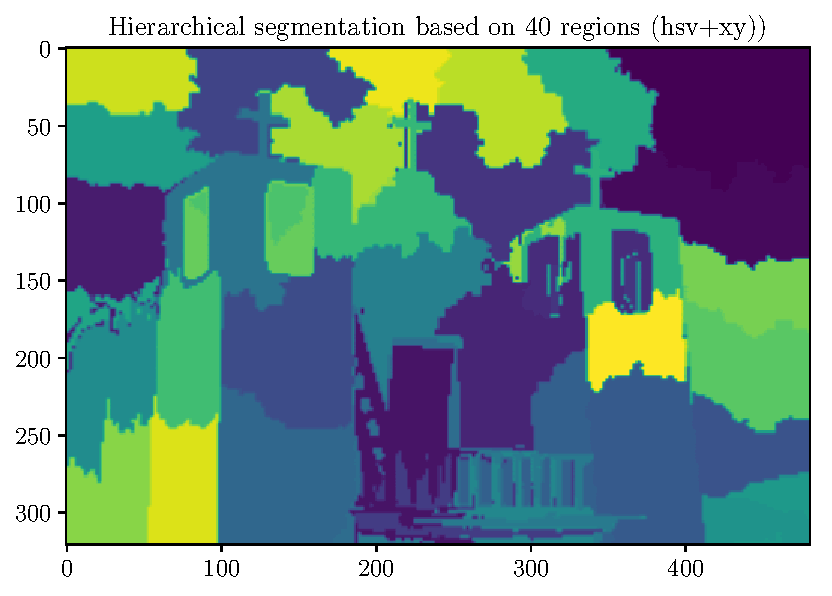
\epsfig{file=./Assets/24063_hierarchical_hsv+xy_40.pdf,width=1.0\linewidth,clip=}
	\caption{Example of Hierarchic segmentation result subject to 40 regions (Spatial information added), notice the smooth noise throughout all the regions by interpolation effects}
	\label{Fig:hier2}
\end{figure}

\begin{figure}[H]
	\centering
	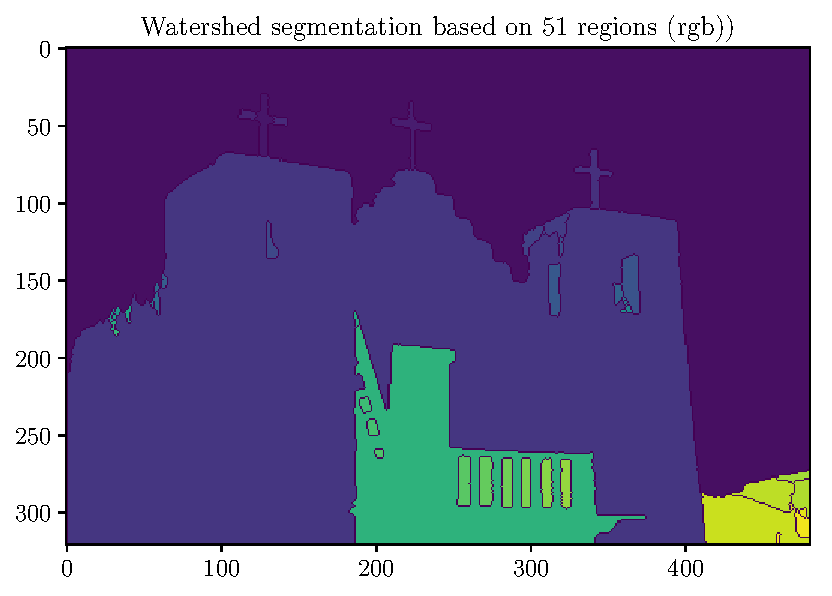
\epsfig{file=./Assets/24063_watershed_rgb_51.pdf,width=1.0\linewidth,clip=}
	\caption{Example of H-Minima Watershed segmentation result subject to 51 regions, notice the well defined contours and regions}
	\label{Fig:water1}
\end{figure}

\begin{figure}[H]
	\centering
	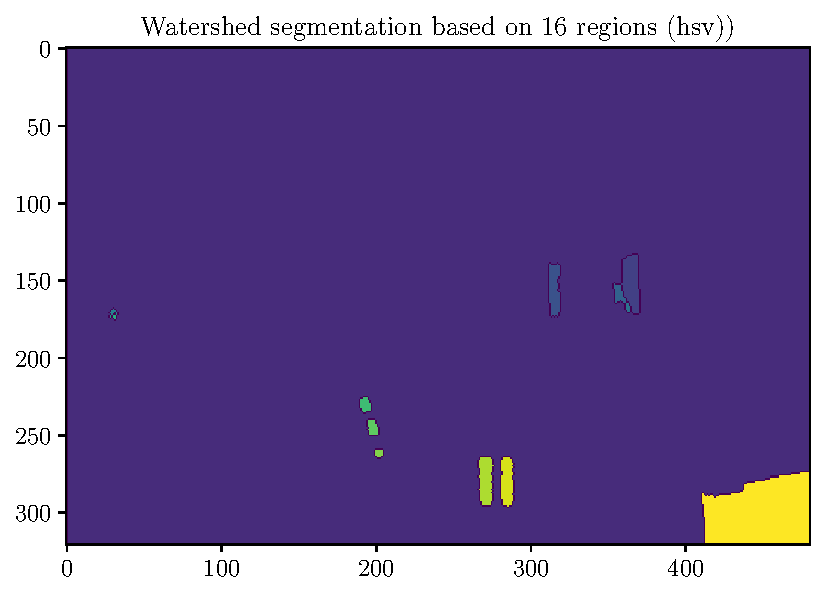
\epsfig{file=./Assets/24063_watershed_hsv_16.pdf,width=1.0\linewidth,clip=}
	\caption{Example of H-Minima Watershed segmentation result subject to 16 regions, notice the disappearance of the main ROI}
	\label{Fig:water2}
\end{figure}



\end{document}
